%% scanner transitions
%% A stub for the re-linking figure.
\begin{figure}
\begin{subfigure}[t]{0.48\textwidth}
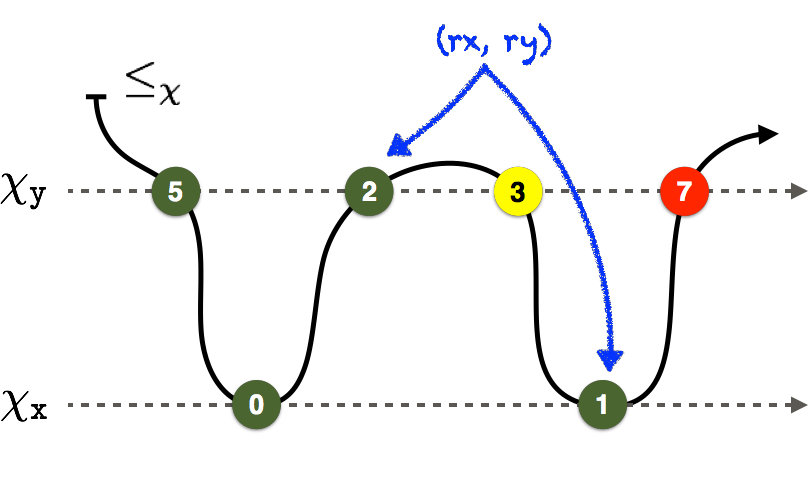
\includegraphics[height=5cm]{res/before-relink-trans}
\caption{\label{fig:relink:before} Before re-link}
\end{subfigure} \hfill
\begin{subfigure}[t]{0.48\textwidth}
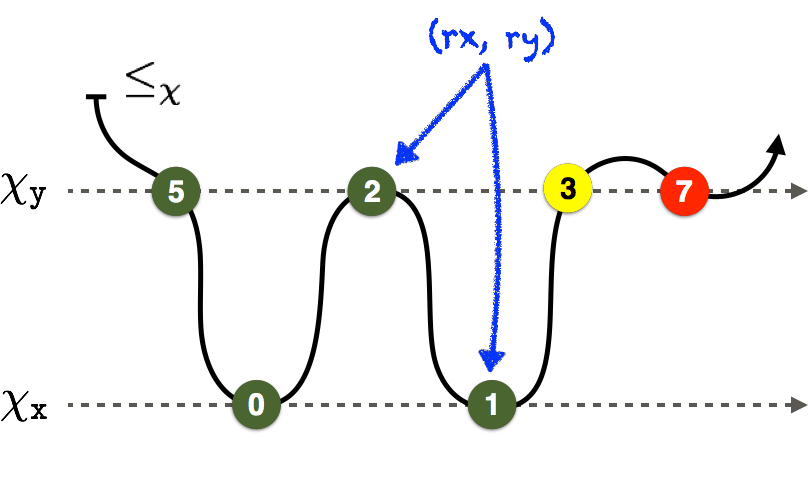
\includegraphics[height=4.5cm]{res/after-relink-trans}
\caption{\label{fig:relink:after} After re-link}
\end{subfigure}%
%
\caption{\label{fig:relink} Atomic re-link: $(rx,ry)$ points to the
  snapshot that will be returned by {\tt scan}}
\end{figure}

\gad{FIX ME: subfigure (b) is incorrectly drawn! 1 and 3 are swapped
  in Real Time as well!!!}

%Fix me: The yellow should be painted red after relink, if we decide
%to go for the (green - red) split for t\left t\right after re-link.
%Though, this would not be stable after we release the lock for scan,
%so why bother. Painting the t|left chain green will suffice, as it
%will be stable.

% Fix me: red marbles have different font colors :(


%\gad{Up to here!}

We next describe the auxiliary code for {\tt scan}.
\[
\begin{array}{l@{\, :\ }l}
%% clear
  \aux{clear}(p) &
      \{\s = \TT,\ \spp = \FF,\ \C = c \}\quad
      \{\s = \TT,\ \spp = \TT,\
      \C = c[\histp \hpts \mathsf{green}] \}\\[3pt]
%% re-link
   \aux{relink}(rx, ry) &
  \!\!\! \begin{array}[t]{l}
    \{\s = \FF, \sx =\TT, \sy = \TT, \C = c, \ordlist = l,\, %
%      t_x = \admissible\ \histx, t_y = \admissible\ \histy, rx = \histx(t_x), ry = \histy(t_y) \}\\
        \hist = h \hunion t_x \hpts (x, rx) \hunion t_y \hpts (y, ry),\\
      \ (t_x = \aux{last\_green}\ \histx \vee
          t_x = \aux{yellow\_of}\ \histx), (t_y = \aux{last\_green}\ \histy \vee
          t_y = \aux{yellow\_of}\ \histy) \}\\
    \{\s = \FF, \sx=\FF, \sy=\FF,%
        \C = c[t_x, t_y \hpts \mathsf{green}],\,\\
      \ \ordlist = \mathsf{if}\ (d = \mathsf{Yes}\ x\ t_r)\
                \mathsf{then}\ \aux{push}\ t_r\, t_y\, l\
                 \mathsf{else\ if}\
                 (d = \mathsf{Yes}\ y\ t_r)\ \mathsf{then}\
                 \aux{push}\ t_r\, t_x\, l\ \mathsf{else}\ l\}\\
  \quad \mbox{where $d = \aux{inspect}\ t_x\, t_y\, l\, \C$}
  \end{array}
\end{array}
\]
%
The procedure $\aux{clear}(p)$ is executed in line~9 simultaneously
with clearing the forward pointer for $p$. In addition to recording
that the scanner passed line~9 by setting the $\spp$ bit, it paints
the subhistory $\histp$ green. Thus, all the previous writes to $p$
will be visible, and hence accounted for in the remaining machinery of
the scan, with their ordering being fixed forever.

Finally, $\aux{relink}$ is the most important among the auxiliary
procedures. It captures the essence of our approach, as it decides how
to change the logical order given in $\ordlist$ (if it needs to change
at all), to justify $(rx,ry)$ as a snapshot.
%
It starts by finding the timestamps $t_x$ and $t_y$ that are
responsible for writing $rx$ and $ry$ into $\histx$ and $\histy$,
respectively. There may be many such timestamps, but we focus on the
ones that are yellow, or last green in the respective subhistories of
their pointer. It follows from invariants (\ref{inv:forward}) and
(\ref{inv:scanner}) that such must exist.
%
Next, $\aux{relink}$ calls the helper procedure $\aux{inspect}$ to
decide if $t_x$ and $t_y$ determine a valid snapshot; that is, there
are no other events between them that make the pair $(rx, ry)$ look
like it is not a snapshot. $\aux{Inspect}$ tests if $t_x < t_y$ and
then makes a decision based on the color of each, and the color of
events between them. The definition has several cases, but we only
describe one here, referring to the example in
Figure~\ref{fig:reorder}. In that figure, we have $rx = 2$, $ry = 1$,
and $t_x$, $t_y$ stand for the events of writing $2$ and $1$,
respectively. Let us assume that both are the last green events in
their respective subhistories, and $t_x < t_y$ in the real
time. However, there is a yellow timestamp in $\histx$ coming afer
$t_x$, corresponding to the write of $3$. Let us name that timestamp
$t'_x$. Because $t_x < t'_x < t_y$, the pair $(rx, ry)$ is not a
snapshot. To make it so, we have to move $t'_x$ out of the way. The
output of $\aux{inspect}$ in this case will precisely be the value
$\mathsf{Yes}\ x\ t'_x$, indicating that $t'_x$ needs to move in the
logical history $\histx$. The move is accomplished by invoking yet
another helper function $\aux{push}$, which reorders $t'_x$ right
after $t_y$ in $\ordlist$.
%
%Notice that the reordering may cause $t'_y$ to jump over 
%several timestamps, thought that is not shown in 
%Figure~\ref{fig:relink}. 
Notice that the move of $t'_x$ respects the invariant that green
timestamps remain fixed. This is a general property of $\aux{relink}$,
which is responsible for stability of $\jleq$.
%
Finally, as the last move in $\aux{relink}$, the color of $tx$ and
$ty$ is changed to green (if it were not so already), thus preventing
future reordering. We can then prove that $(rx, ry)$ will be a valid
snapshot wrt.~$L$ under any interference.


\begin{comment}
%
$\aux{relink}$ works as follows: first, the auxiliary function 
$\mathsf{decide}$ checks $l$ to see if $t_x$ and $t_y$ form a valid 
snapshot, in which case it will return $\mathsf{No}$ and then 
$\ordlist = l$, else it will return $\mathsf{Yes}\ p\ t_r$, indicating 
that there is a miss and that $t_r \in \hist_{p}$--- and is such that 
$t_r \leq t_{\neq p}$ ---should be {\it pushed} in $\ordlist$ past 
$t_{\neq p}$, the latter being $t_y$ if $p=x$, and vice 
versa. Finally, the returned timestamps are painted green.



In Figure~\ref{fig:relink}, we revisit the example from
Section~\ref{sc:overview}, adding the colors to the time-stamps. There
we see in Figure~\ref{fig:relink:before} that $(rx,ry)$ points to
$(2,1)$ and both timestamps are green. We notice that there is a
yellow in between, $\mathsf{yellow}\, \histx$.  In
Figure~\ref{fig:relink:after}, we see that it has been pushed after
$ry$.

$\aux{relink}$ works as follows: first, the auxiliary function 
$\mathsf{decide}$ checks $l$ to see if $t_x$ and $t_y$ form a valid 
snapshot, in which case it will return $\mathsf{No}$ and then 
$\ordlist = l$, else it will return $\mathsf{Yes}\ p\ t_r$, indicating 
that there is a miss and that $t_r \in \hist_{p}$--- and is such that 
$t_r \leq t_{\neq p}$ ---should be {\it pushed} in $\ordlist$ past 
$t_{\neq p}$, the latter being $t_y$ if $p=x$, and vice 
versa. Finally, the returned timestamps are painted green.

We clarify how $\mathsf{decide}$ works: without any loss of
generality, assume $t_x \tleq t_y$. The pre-condition of
$\aux{relink}$ says $t_x$ and $t_y$ are, respectively, the last green
or yellow timestamps of $\histx$ and respectively $\histy$. From the
latter facts facts and Invariant~\ref{inv:redzone}, we know that every
timestamp in the chain from $t_x \tleq t_y$ will be green or yellow
and there will be, at most, two yellow timestamps, one for each
$\histx$ and $\histy$. Then, if $t_x$ is yellow, $\mathsf{decide}$
will return $\mathsf{No}$-- if there are further elements in $\histx$,
they will be in the red tail, and outside the chain-- e.g. the token 7
in Figure~\ref{fig:relink}. Now, if $t_x$ is green and there is no
yellow key in $\histx$, $\mathsf{decide}$ will return
$\mathsf{No}$. If there is, we need to compare it with $t_y$: if
$\mathsf{yellow}\ \histx \tle t_y$, as in Figure~\ref{fig:relink},
$\mathsf{decide}$ will return $\mathsf{Yes}\ x\
(\mathsf{yellow}\, \histx)$ and the latter will be pushed right after
$t_y$ in \ordlist-- $\mathsf{push}$ implements the pointer-swing-like
manipulation on $l$. Last, if $ t_y \tle \mathsf{yellow}\ \histx$
there will be no $\mathsf{push}$ either.

\end{comment}

%% \gad{The figure might change to include the red-zone invariant as well,
%%   as the endpoints if we need to}. Here give a proof-sketch on how
%% re-link satisfies the invariants.
